
%(BEGIN_QUESTION)
% Copyright 2006, Tony R. Kuphaldt, released under the Creative Commons Attribution License (v 1.0)
% This means you may do almost anything with this work of mine, so long as you give me proper credit

Shown here is the mechanism for a simplified (no amplifying relay, no bias spring) proportional-only pneumatic controller:

$$\includegraphics[width=15.5cm]{i01542x01.eps}$$

Explain how this controller mechanism functions, being sure to include the concept of {\it negative feedback} in your explanation.

\vskip 10pt

\filbreak

Suppose this pneumatic controller developed a problem: the short tube connecting to the feedback bellows becomes completely plugged.  This does not allow the feedback bellows to sense air pressure at the nozzle:

$$\includegraphics[width=15.5cm]{i01542x02.eps}$$

Describe and explain the effect this tube blockage will have on controller behavior.

\vskip 10pt

\filbreak

Now suppose the same tube were only {\it partially} plugged, with the effect of slowing down air passage through it, so that the bellows pressure lags behind the nozzle pressure in time:

$$\includegraphics[width=15.5cm]{i01542x04.eps}$$

\underbar{file i01542}
%(END_QUESTION)





%(BEGIN_ANSWER)

I will answer the question of total tube blockage with another question: what will happen in the following operational amplifier circuit if the feedback resistor fails open?

$$\includegraphics[width=15.5cm]{i01542x03.eps}$$

Given a partial blockage, the controller will ``over-react'' to sudden changes in either PV or SP, then settle out at the normal output signal value expected as a proportional controller.

%(END_ANSWER)





%(BEGIN_NOTES)



%INDEX% Control, proportional: pneumatic force-balance controller

%(END_NOTES)


